\begin{frame}{Installation}
  To install the the EuXFEL beamer theme you need to do the following
  \begin{itemize}
  \item Download the EuXFEL beamer package
  \item Follow the \href{https://docs.xfel.eu/share/proxy/alfresco/api/node/content/workspace/SpacesStore/92e260f4-e0a7-4463-a812-40a180bd6e75/IN-2012-003-01_LaTeX_User_Guide.pdf?a=true}{\colorbf{European XFEL LaTeX User Guide}} on how to install latex packages.
  \end{itemize}
  \begin{block}{On Linux}
    Extract the package file to\\
    \centerline{\textit{$\sim$/texmf/tex/latex/}}
    and run
    \centerline{ \textit{texhash   $\quad\sim$/texmf/tex/latex/ }}
    in your console.
  \end{block}
\end{frame}

\begin{frame}[fragile]{Usage}
  Start your Latex beamer file with:
  \begin{block}{}
    \begin{verbatim}
\documentclass[10pt,aspectratio=169]{beamer}
\mode<presentation> {
  \usetheme{EuXFEL}
  \usecolortheme{EuXFEL}
}

\end{verbatim}
  \end{block}
\end{frame}

\begin{frame}{Frame Title}
  \begin{itemize}
  \item \lipsum[2][2]
    \begin{itemize}
    \item \lipsum[3][2]
      \begin{itemize}
      \item \lipsum[4][2]          
      \end{itemize}
    \end{itemize}
  \end{itemize}
  
  \begin{block}{Block Title}
    Consider a \colorbf{function} $\rho(r,\phi)$ such that
    \begin{equation}
      \label{eq:1}
      \int_{\gamma} \rho(r,\phi)\, drd\phi=\frac{\pi}{2}
    \end{equation}
  \end{block}
\end{frame}


\begin{frame}{Multiple Columns}
  \begin{columns}[onlytextwidth]
    \begin{column}{0.5\textwidth}
      \lipsum[6][1-4]\\      
      \begin{center}
        \def\ry{.6}        % vertical radius outer ellipse
        \def\kry{\ry*.5} % vertical radius inner ellipse
        \def\rx{.3}        % horizontal radius outer ellipse
        \def\krx{\rx*.5} % horizontal radius inner ellipse

        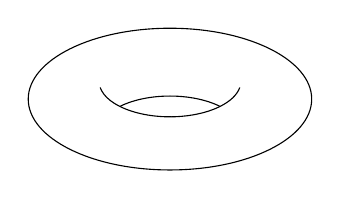
\begin{tikzpicture}[scale=3]
          % outer ellipse
          \draw ([shift=(0:{\ry} and \rx)]0,0) arc (0:360:{\ry} and \rx);
          % hole (inner ellipse)
          \draw ([shift=(190:{\kry} and \krx)]0,\kry*.25) arc (190:350:{\kry} and \krx);  
          \draw ([shift=(315:{\kry} and \krx)]0,\kry*.25) arc (45:135:{\kry} and \krx);
        \end{tikzpicture}
      \end{center}
      \end{column}
      \begin{column}{0.5\textwidth}
        \begin{enumerate}
        \item \lipsum[6][6]
        \item \lipsum[6][7]
        \item \lipsum[6][8]
        \item \lipsum[6][9]
        \end{enumerate}
        \begin{block}{\centering Something very\\ important!}
          \vspace{-3cm}
        \end{block}
      \end{column}
  \end{columns}
\end{frame}